\documentclass[10pt,a4paper]{article}
\usepackage[utf8]{inputenc}
\usepackage{amsmath}
\usepackage{amsfonts}
\usepackage{amssymb}
\usepackage{graphicx}
\usepackage{color}
\usepackage{float}
\usepackage{gensymb}

\usepackage{listings}
\usepackage[ampersand]{easylist}
\usepackage{setspace}
\usepackage{makeidx}
\usepackage{wrapfig}
\usepackage{etoolbox}

\usepackage{eurosym}
\usepackage{siunitx}
 
\usepackage{fancyhdr}

\usepackage{titlesec}

\setcounter{secnumdepth}{4}

\titleformat{\paragraph}
{\normalfont\normalsize\bfseries}{\theparagraph}{1em}{}
\titlespacing*{\paragraph}
{0pt}{3.25ex plus 1ex minus .2ex}{1.5ex plus .2ex}
 
\pagestyle{fancy}
\fancyhf{}
\rhead{Amsterdam university of applied sciences}
\lhead{Technical Document}
\rfoot{Page \thepage}


\usepackage{draftwatermark}
\SetWatermarkText{}
\SetWatermarkScale{5}

\definecolor{codegreen}{rgb}{0,0.6,0}
\definecolor{codegray}{rgb}{0.5,0.5,0.5}
\definecolor{codepurple}{rgb}{0.58,0,0.82}
\definecolor{backcolour}{rgb}{0.95,0.95,0.92}
\usepackage{listings}
\lstdefinestyle{cstyle}{
    backgroundcolor=\color{backcolour},   
    commentstyle=\color{codegreen},
    keywordstyle=\color{magenta},
    numberstyle=\tiny\color{codegray},
    stringstyle=\color{codepurple},
    basicstyle=\footnotesize,
    breakatwhitespace=false,         
    breaklines=true,                 
    captionpos=b,                    
    keepspaces=true,                 
    numbers=left,                    
    numbersep=5pt,                  
    showspaces=false,                
    showstringspaces=false,
    showtabs=false,                  
    tabsize=2
}
\lstset{ %
    backgroundcolor=\color[RGB]{250,250,250},   % choose the background color; you must add \usepackage{color} or \usepackage{xcolor}
    basicstyle=\ttfamily,        % the size of the fonts that are used for the code
    breakatwhitespace=false,         % sets if automatic breaks should only happen at whitespace
    breaklines=true,                % sets automatic line breaking
    captionpos=b,                    % sets the caption-position to bottom
    commentstyle=\color[RGB]{0,128,0},    % comment style
    extendedchars=true,              % lets you use non-ASCII characters; for 8-bits encodings only, does not work with UTF-8
    frame=lines,                    % adds a frame around the code
    keepspaces=true,                 % keeps spaces in text, useful for keeping indentation of code (possibly needs columns=flexible)
    keywordstyle=\color{blue},       % keyword style
    language=C,                 % the language of the code
    numbers=left,                    % where to put the line-numbers; possible values are (none, left, right)
    numbersep=10pt,                   % how far the line-numbers are from the code
    numberstyle=\color[RGB]{50,50,50}, % the style that is used for the line-numbers
    rulecolor=\color{black},         % if not set, the frame-color may be changed on line-breaks within not-black text (e.g. comments (green here))
    showstringspaces=false,          % underline spaces within strings only
    showtabs=false,                  % show tabs within strings adding particular underscores
    stepnumber=1,                    % the step between two line-numbers. If it's 1, each line will be numbered
    stringstyle=\color[RGB]{128,0,128},     % string literal style
    tabsize=2,                       % sets default tabsize to 2 spaces
    title=\lstname                   % show the filename of files included with \lstinputlisting; also try caption instead of title
}
\renewcommand{\lstlistingname}{Code}% Listing -> Algorithm
\renewcommand{\lstlistlistingname}{Codes}

\graphicspath{ {./images/} }

\begin{document}
\begin{titlepage}
    \centering
    \vfill
    {\Large

    Swarming Module\\

   
    {\small Technical Document}\\
    {\small Version 1.0}\\
    {\small \today}\\
        
        \vskip2cm
        {\small M. van Wilgenburg, W. Mukhtar, E. van Splunter, M. Siekerman, T. Zaal and M. Visser}\\
    }    
    \vfill
%    \includegraphics[width=1\textwidth]{WireS4}
    
    \vfill
    \vfill
\end{titlepage}

\newpage

\listoffigures
\newpage

\listoftables
\newpage

\tableofcontents
\newpage

\section{Abstract}

\section{Introduction}
This document describes the technical aspect of the "Swarming Module". This module is developed by students of the Amsterdam University of Applied sciences in collaboration with the Delft University of Technology.   This project is a part of a running research program that is looking into the benefits of swarming compared to "standard" approaches, which would be one bigger and more complex robot doing all the work. Finally this program looks at the applications swarming might have on Mars. 

This project contributes to the program by developing a so called "Swarming Module". This module will allow units in a swarm to determine the relative location to one another. When the units know their relative location, multiple complex tasks can be achieved like: path finding, payload transfer from one unit to another, autonomous recharging, and much more. 

\subsection{Swarming}
The term "Swarming" is still a wide concept which is not well defined. However most people agree the following criteria should be met before a group of robots can be defined as a swarm:

\begin{itemize}
	\item Autonomy - It is required that the individuals that make up 	the swarm-robotic system are autonomous robots. They are able to 		physically 		interact with the environment and affect it\cite{swarmintelligence}.
	\item Large number - A large number of units is required
	as well, so the cooperative behavior (and
	swarm intelligence) may occur. The minimum number
	is hard to define and justify. The swarm-robotic
	system can be made of few homogeneous groups of
	robots consisted of large number of units. Highly heterogeneous
	robot groups tend to fall outside swarm
	robotics.\cite{swarmintelligence}
	\item Limited capabilities - The robots in a swarm
	should be relatively incapable or inefficien on their
	own with respect to the task at hand.\cite{swarmintelligence}
	\item Scalability and robustness - A swarm-robotic
	system needs to be scalable and robust. Adding the
	new units will improve the performance of the overall
	system and on the other hand, loosing some units will
	not cause the catastrophic failure.\cite{swarmintelligence}
	\item Distributed coordination - The robots in a swarm
	should only have local and limited sensing and communication
	abilities. The coordination between the
	robots is distributed. The use of a global channel for
	the coordination would influence the autonomy of the
	units.\cite{swarmintelligence}
\end{itemize}

The swarming module provides the information so the last criteria 'Distributed coordination' can be met. The specifications must be formulated so they meet the criteria of "Large numbers", and "Scalability and robustness". It would be preferable to make the swarm endlessly scalable, however hardware limitations will probably hinder this. 

\subsection{Specifications}
Before the features of the Swarming module are specified, swarming itself should be specified further. In section 1 of the research document this is done by creating a set of realistic scenarios. From this specifications like: minimal distance, maximal distance, maximum number of units, and precision are derived. These specifications are summarised in Table \ref{smrange} and Table \ref{specunits}. 

\begin{table}[h]
\centering
\resizebox{\textwidth}{!}{%
\begin{tabular}{|l|l|l|}
\hline
                     & \textbf{Close range (0 - 3 m)} & \textbf{Long range (3 - 25 m)} \\ \hline
Dead zone distance    & 0,015 meters                   & 2 meters                      \\ \hline
Deviation (distance) & +/- 9\%                         & +/- 1 meter                   \\ \hline
Angle Resolution     & 45\%                            & -                             \\ \hline
Update frequency     & 40 Hz                           & 1 Hz                           \\ \hline
\end{tabular}%
}
\caption{Swarming localization specifications}
\label{smrange}
\end{table}

\begin{table}[h]
\centering
\resizebox{\textwidth}{!}{%
\begin{tabular}{|l|l|l|l|l|}
\hline
 & \textbf{minimum} & \textbf{maximum} & \textbf{maximum (close range)} & \textbf{Preferred (demonstration)} \\ \hline
Number of Units & \multicolumn{1}{c|}{3} & \multicolumn{1}{c|}{$\infty$} & \multicolumn{1}{c|}{130} & \multicolumn{1}{c|}{6 to 12} \\ \hline
\end{tabular}%
}
\caption{Specifications number of units}
\label{specunits}
\end{table}


The choice is made to divide the the specifications for localization into two categories: Close range, and long range. This choice was made because at close range more precision precision is needed to prevent the robots from crashing into each other. While at long range the localization will be used not to loose the swarm. The maximum number at close range is derived from the theoretical number of units that can physically fit in a 3 meter radius. And the preferred number of units for demonstration purpose is used to set a goal for the project. For further clarification how these specifications are determined see chapter one of the research document.

\section{Research}
This section will a summary of the findings during the research phase. From the full version of the research done during this project we refer to the "Research Document". \\
The research is split up in the following different subjects: Localization, Hardware communication protocol, Software communication protocol.

\subsection{Localization}
This section will cover the following subjects: Relative distance measurement, and Relative angle measurement. With these two variables the relative location of other units can be derived. 

\subsubsection{Relative distance}
Before any calculations can be done to derive the angle of other units a distance must first be determined. The first choice that has to be made is what type of signal is used to do this. The most commonly used type of signal to measure distance are radio waves, which propagate with the speed of light. Hardware to measure these  signals over short distances, would require clock-speeds of in the GHz, hence be expensive and unstable. Therefore the choice is made to use acoustic signals to measure the distance. This drastically lowers the requirements for the hardware that detects the signal.

Now that this is established there are still two ways to implement a distance measurement. These are: Time of flight (TOF), and Received signal strenght (RSSI). During experiments (found in section 4.3 of the Research document) we found that the received amplitude of the acoustic signal was not proportional to the distance. We also found that the signal was still well defined over the specified distance of three meters. Because of this the signal can be detected and used for TOF.

A system is proposed that combines the two signals (radio and acoustic) in one system. Swarming modules each get their place in time to send their acoustic signal. At the moment the module starts sending the acoustic signal, he sends a message over the radio communication channel saying "im going to send my signal", the radio signal arrives close to instantly compared to the acoustic signal. At this point all the other modules start their timers, and stop them when the acoustic signal arrives a few moments later. The distance can now be calculated to multiply the time with the speed of sound.


\subsection{Relative angle}
Determining the relative orientation with respect to each other can be done in various ways. some methods involve larger limitations than others. In general angular measurements are done using goniometric equations. It was found that calculating the angle with a single measuring point on every swarming module has one big problem. Because geometric functions are used to calculate the angle, there will always be two solutions to the equation (see figure \ref{circle} and section 3.1.1 of the Research document). To solve this the units would have to move and recalculate again to get the right answer. This would limit the units in their movement and functionality and is non desirable.

\begin{figure}[H]
\centering
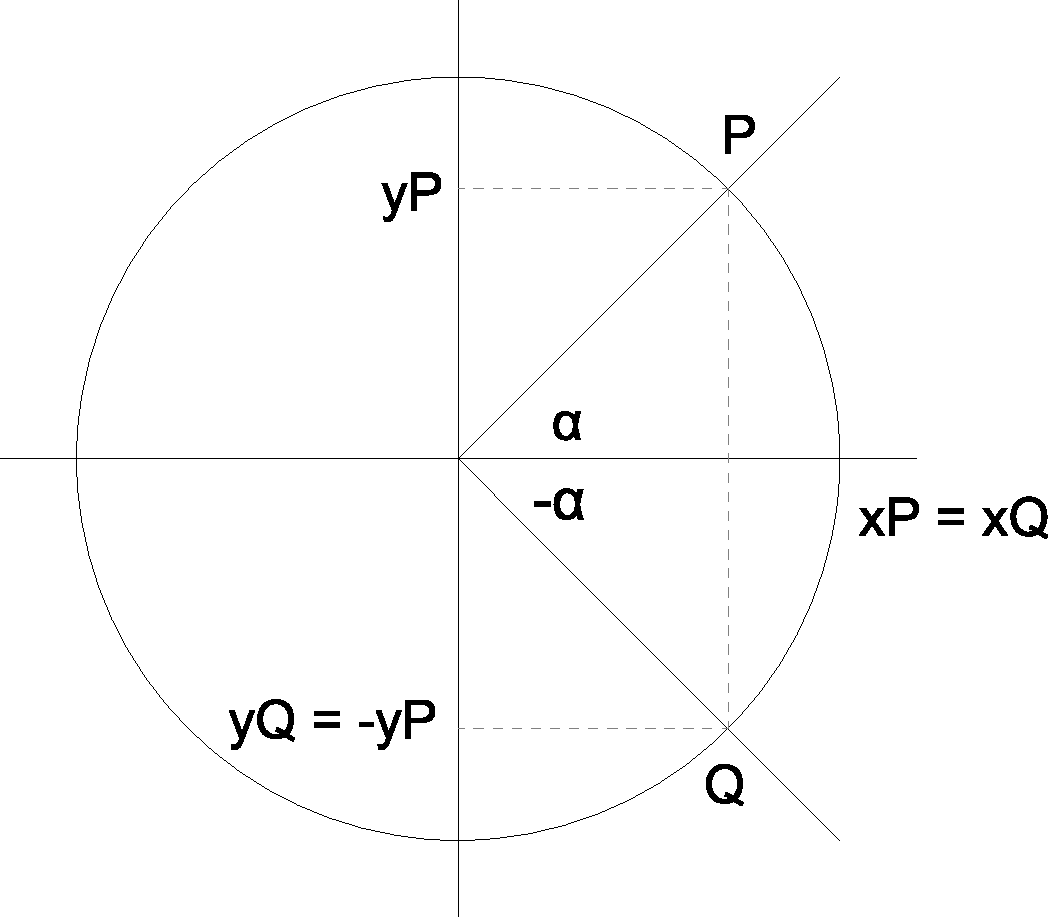
\includegraphics[width=0.7\textwidth]{Cirkel.pdf}
\caption{Unit circle where points P and Q are mirrored on the X-axes}
\label{circle}
\end{figure}

\begin{equation}
Because\ Xp = Xq,\ cos(-\alpha) = cos(\alpha)\ applies
\end{equation}

\begin{equation}
Because\ Yq = -Yp,\ sin(-\alpha) = -sin(\alpha)\ applies
\end{equation}


To solve this problem a system is proposed with three or more acoustic receivers with a predefined distance between them. Using the difference in time and the predefined distance, the angle can be calculated with only one solution. This method is shown in figure \ref{trigonometry}.

\begin{figure}[H]
\centering
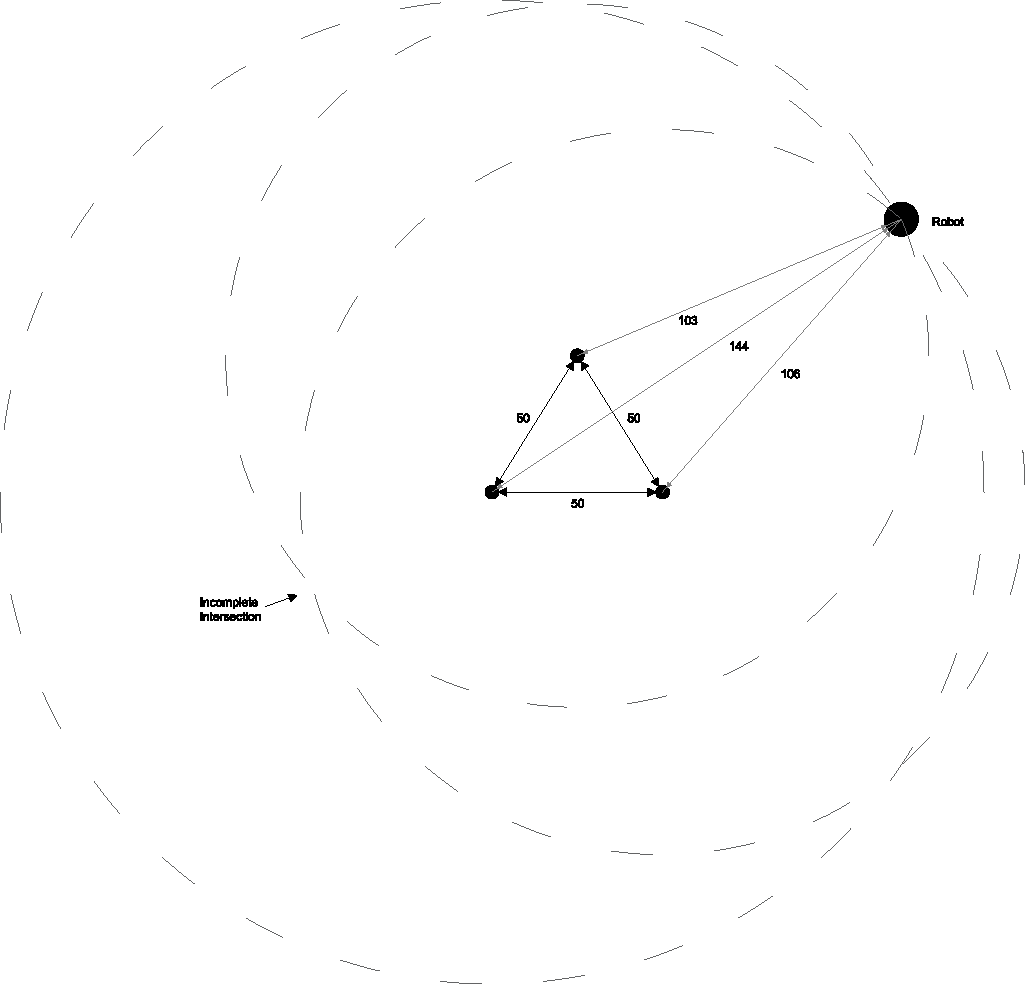
\includegraphics[width=1\textwidth]{trigonometry.pdf}
\caption{Angle determination using trigonometry}
\label{trigonometry}
\end{figure}

\subsection{Acoustic Sensing}
In this section the behaviour of acoustic sensing will be researched. This was done in real life experiments using a microphone, speaker and scope to analyse the received signals. During experiments the following points where analysed:

\begin{itemize}
\item Sound has to spread in every direction (omnidirectional).
\item The received acoustic signal has to be well defined within a minimal distance of 3 meters.
\item What frequency shows the best results.
\end{itemize}

More details about the experiment and the setup are shown in section 4 of the Research document. The first experiment had the speakers facing the microphone directly, this was clearly the best situation, higher frequencies showed higher amplitude and the signal was well defined. However the most ideal situation would be for one speaker to be omnidirectional instead of having to use multiple speakers.  \\
Another test was done with the speaker and microphone both facing upwards. It was observed that higher frequency sound (around 5 kHz) becomes more directional. The best results were achieved around 3 - 4 kHz, this was the point where the highest amplitude was achieved and the minimum distance of three meters was easily met.


\subsection{Functional specifications}

\subsubsection{Wireless communication} 

The specifications of the wireless communication are  discussed in our framework, but will be shortly summarized. 

\begin{table}[H]
\centering
\caption{Wireless communication module}
\label{wirelesscommunication}
\begin{tabular}{|l|l|}
\hline
Module    & Wireless communication module \\ \hline
Input  & \begin{tabular}[c]{@{}l@{}}Communication with the system\\ Communication with the other robots in the swarm          
\end{tabular}   \\ \hline
Output & \begin{tabular}[c]{@{}l@{}}Communication with the system\\ Communication with the other robots in the swarm         
\end{tabular}   \\ \hline
Functions   & \begin{tabular}[c]{@{}l@{}}establishes the communication between the modules swarm \\ Obtains information regarding the distance between the different robots\end{tabular}            \\ \hline
\end{tabular}
\end{table}

To communicate between different units a communication network should
be set up with a common protocol . In addition, the protocol must be able to
provide additional information such as localization. See Table \ref{wirelesscommunication}. 

\subsubsection{Central control unit}

The central control unit handles all communication between the various modules that are present on the robot. See Table \ref{control}

\begin{table}[H]
\centering
\caption{Central control unit}
\label{control}
\begin{tabular}{|l|l|}
\hline
Module    & Central control unit \\ \hline
Input  & All information from the system  \\ \hline
Output & All control of the modules in the robot \\ \hline
Functions  & All the communication comes together and controls the inputs and outputs            \\ \hline
\end{tabular}
\end{table}





\subsection{Specifications}

\subsubsection{Wireless communication}

In Table \ref{wcm} a more detailed version of the specifications are written down. From these specifications the module will be implemented as is shown in the next section. 

\begin{table}[H]
\centering
\caption{Wireless communication module}
\label{wcm}
\begin{tabular}{|p{1,5cm}|p{9,5cm}|}
\hline
Module   & Wireless communication module                                       \\ \hline
Input    & 5 VDC\\ 
        & Swarm data\\
        & RF signal                                              \\ \hline
Outputs  & RF signal                                           \\ 
& Swarm data \\ \hline
Function & Processes information to and from other swarm modules. Transmission speed is not defined yet. The transmission range must be around 100 meters or more. \\ \hline
\end{tabular}
\end{table}

\subsubsection{Central operating unit}
The central operating unit processes data from the sensors and swarm network. This unit uses the external wireless swarm communication, the local communication bus and the debug interface as an communication channel. The local communication bus uses a TWI (Two Wire Interface) protocol and is used for the communication with the robots peripherals i.e. actuators. The debug interface of the central operating unit uses an UART protocol to communicate with external systems for debug purposes.

\begin{table}[H]
\centering
\caption{Central operating unit}
\label{cou}
\begin{tabular}{|p{1,5cm}|p{9,5cm}|}
\hline
Module   & Central operating unit                                        \\ \hline
Input    & 3,3 VDC \\
         & Data streams (TWI, UART)                                           \\ \hline
Outputs  & Data streams (TWI, UART)                                             \\ \hline
Function & Calculates the relative position to other swarming modules. Distributes local and external data streams. Analyses and uses sensor information.\\ \hline
\end{tabular}
\end{table}

\subsection{Implementation}

\subsubsection{Central operating unit}

In Table \ref{cou} the basic specifications of the AtXmega128A4U are shown. This is the microcontroller used in as the central operating unit. The microcontroller from Atmel complies with all the specifications. An overview of all the specification can be found on the website of Atmel. 


\begin{table}[]
\centering
\caption{Central operating unit}
\label{cou}
\begin{tabular}{|l|l|}
\hline
\textbf{Parameter}			& \textbf{Value} \\ \hline
Flash (kBytes):             & 128 kBytes \\ \hline
Pin Count:                  & 44         \\ \hline
Max. Operating Freq. (MHz): & 32 MHz     \\ \hline
CPU:                        & 8-bit AVR  \\ \hline
Max I/O pins:               & 34         \\ \hline
USB Interface:              & Device     \\ \hline
SPI:                        & 7          \\ \hline
TWI (I2C):                  & 2          \\ \hline
UART:                       & 5          \\ \hline
ADC Channels:               & 12         \\ \hline
ADC Resolution (bits):      & 12         \\ \hline
ADC Speed (ksps):           & 2000       \\ \hline
DAC Channels:               & 2          \\ \hline
SRAM (kBytes):              & 8          \\ \hline
EEPROM (Bytes)              & 2048       \\ \hline
Operating Voltage (Vcc):    & 1.6 to 3.6 \\ \hline
\end{tabular}
\end{table}

\subsubsection{Functions}

The Central operating unit handles multiple functions to make the group of robots a swarm. Those functions will be explained in this section.
There are four major functions that are implemented in the microcontroller. Controlling communication that goes in and out, storage and maintain data, calculating the population of the swarm and send and receive message that are used for localization. The 

\subsubsection{Wireless communication}

\begin{table}[]
\centering
\caption{Swarmbee LE module} 
\label{SwarmbeeLE}
\resizebox{\textwidth}{!}{%
\begin{tabular}{|ll|}
\hline
\multicolumn{1}{|l|}{\textbf{Parameter}}                                                                                                 & \textbf{Value}                                                                                                                 \\ \hline
\multicolumn{1}{|l|}{Frequency range}                                                                                                    & ISM band 2.4 GHz (2.4 - 2.4835 GHz)                                                                                            \\ \hline
\multicolumn{1}{|l|}{Modulation}                                                                                                         & Chirp Spread Spectrum (CSS)                                                                                                    \\ \hline
\multicolumn{1}{|l|}{Transmission modes}                                                                                                 & \begin{tabular}[c]{@{}l@{}}80 MHz, 1 Mbps or 250 Kbps\\ (80/1 or 80/4 mode)\end{tabular}                                       \\ \hline
\multicolumn{1}{|l|}{TOA capture accuracy}                                                                                               & \textless 1 ns (better than 30 cm)                                                                                             \\ \hline
\multicolumn{1}{|l|}{Typical air time per ranging cycle}                                                                                 & 1.8 ms                                                                                                                         \\ \hline
\multicolumn{1}{|l|}{RF output power}                                                                                                    & configurable - 22 t0 16 dBm                                                                                                    \\ \hline
\multicolumn{1}{|l|}{RF sensitivity}                                                                                                     & \begin{tabular}[c]{@{}l@{}}-89 dBm typ. @80/1 mode\\ -95 dBm typ. @80/4 mode\end{tabular}                                      \\ \hline
\multicolumn{1}{|l|}{RF interface}                                                                                                       & 50 Ohm RF port (for external antenna)                                                                                          \\ \hline
\multicolumn{1}{|l|}{Host interface (UART)}                                                                                              & 500bps $\sim$ 2 Mbps                                                                                                           \\ \hline
\multicolumn{1}{|l|}{Power supply}                                                                                                       & 3 - 5.5 V                                                                                                                      \\ \hline
\multicolumn{1}{|l|}{Max. supply voltage ripple}                                                                                         & 20 mVpp                                                                                                                        \\ \hline
\multicolumn{1}{|l|}{Active power consumption*}                                                                                          & 120 mA during transmission, 60 mA during receive in 80/1 mode                                                                  \\ \hline
\multicolumn{1}{|l|}{Power consumption in sleep mode*}                                                                                   & 5.5 mA (transceiver disabled, all peripherals on)                                                                              \\ \hline
\multicolumn{1}{|l|}{Power consumption in snooze mode*}                                                                                  & 4.5 \si{micro}A (transceiver disabled, all peripherals off, wake-up by timer)                                                           \\ \hline
\multicolumn{1}{|l|}{Power consumption in nap mode**}                                                                                    & \begin{tabular}[c]{@{}l@{}}4.5 $\sim$ 600 \si{micro}A (transceiver disabled, all peripherals off, wake-up by \\ interrupt)\end{tabular} \\ \hline
\multicolumn{1}{|l|}{Power consumption in deep-sleep mode*}                                                                              & \textless 1 \si{micro}A (device completely disabled)                                                                                    \\ \hline
\multicolumn{1}{|l|}{Operating temperature range}                                                                                        & -30 - 85 $^{\circ}$C                                                                                                                    \\ \hline
\multicolumn{1}{|l|}{Dimensions}                                                                                                         & 40 mm x 24 mm x 3.5 mm                                                                                                         \\ \hline
\multicolumn{1}{|l|}{Weight}                                                                                                             & 7 g                                                                                                                            \\ \hline
\begin{tabular}[c]{@{}l@{}}*Power consumption in all modes is \\ measured at 20$^{\circ}$C, 3.3 V.\end{tabular}                                   &                                                                                                                                \\ \hline
\begin{tabular}[c]{@{}l@{}}**Power consumption in nap mode \\ depends  on interrupt sources (GPIO \\ pins or MEMS or both).\end{tabular} &                                                                                                                                \\ \hline
\end{tabular}%
}
\end{table}

For the wireless communication module the most important function is that it can transmit information over atleast 100 meters. The speed of de communication is not defined yet. The Swarmbee LE module will be used for the wireless communication. Its uses the ISM band, 2.4 GHz to transmit the data. The maximum range of the module relies on the environment in which it is used. Under ideal conditions the Swarmbee can reach a distance of 1200 meters. It depends on how many obstacles, reflections and interference there is to disturb the signal. An experiment from Nanotron showed that until a range of 150 meters the ranging success rate is about 100%. The host interfaces uses UART
with a transmission speed of 155 kbps. Transmitting data between the swarm modules can be configured with a speed of 250 Kbps or 1 Mbps. This module fits all the specifications and is suitable for the use of wireless communication.

\newpage



\section{Bibliografie}
\bibliography{references}
\bibliographystyle{IEEEtran}



\end{document}
